\chapter{Fourier Transformation}
\label{Fourier Transformation}


\begin{center}
\begin{figure}[h!]
\tikzset{concept/.append style={fill={none}}}
\begin{tikzpicture}
  \path[mindmap,concept color=black,text=black]
	node[concept] {FFT uebung}
	[clockwise from=0]
	child[concept color=green!50!black] {
	node[concept] {schuluebung v. letzem Mal}
	}
	child[concept color=green!50!black] {node[concept] {pd parxis}
		child[concept color=green!50!black] {node[concept] {send/receive}}
		child[concept color=green!50!black] {node[concept] {initialisierung}}
		}
	child[concept color=blue] {
	node[concept] {hauptteil FFT}
	[clockwise from=-90]
		child[concept color=orange] { node[concept] {theorie} }
		child[concept color=red] { node[concept] {praxis} 
			child[concept color=red] { node[concept] {spectrum display} }
			child[concept color=red] { node[concept] {fft filter} 
				child[concept color=red] { node[concept] {random filter} }
				}
			child[concept color=red] { node[concept] {fft reverb} }
			child[concept color=red] { node[concept] {pitch shift} }
			}
	}

;
\end{tikzpicture}
\caption{Lecture Contents: Fourier Transformation}
\end{figure}
\end{center}

\section{Notizen}

vorbereitung:\\
Eulers identity, complex numbers.



Initialisierung
Fourier transformation.
Spectral filter
Spectral Reverb, delay.
Windowing
Convolution,
evtl. cross correlation
freq. crossover
spectral synyth,
spectraum display.


evtl auch:
\begin{itemize}
	\item send / receive, send / receive bei gui objekten.
	\item initialisierung
	\item 
\end{itemize}


Diskretes Signal -> Periodisches Spectrum \\
Periodisches Signal -> Diskretes Spectrum

gute referenz:
http://jackschaedler.github.io/circles-sines-signals


% fftuebung
% beiwerk:
	% initialisierung
	% send/receive
% schuluebung von letzem mal
% hauttteil fft
	% theorie	> geschichte
	% praxis
		% spectrum display
		% fft filter
			% nomral
			% random
		% fftdelay
		% fft reverb
		% pitch shift


\section{Fourier Transformation}

Geschichte:
Bernoulli, Euler, Gauß, Fourier

Eulers identität:
\begin{equation}
	e ^{ix} = cos(x)+i \cdot sin(x)
\end{equation}

Fourier Transformation:\\
\begin{equation}
	X(f)= \mathcal{F} \{x(t)\} = \int_{-\infty}^\infty \! x(t) e^{-j2\pi ft} \, \mathrm{d}t
\end{equation}

Inverse Fourier Transformation:\\
\begin{equation}
	x(t)= \mathcal{F}^{-1} \{X(f)\} = \int_{-\infty}^\infty \! X(f) e^{j2\pi ft} \, \mathrm{d}f
\end{equation}

\begin{figure}[h]
	\begin{center}
		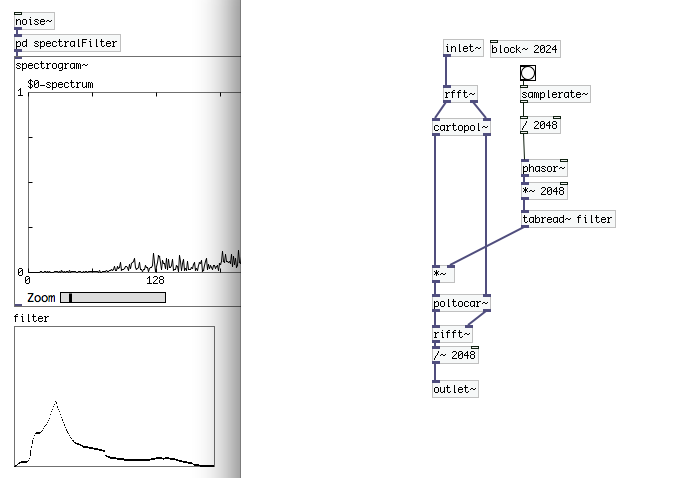
\includegraphics[width = 14cm]{img/spectralFilter.png}
		\caption{spectralFilter.pd}
		\label{fig:spectralFilter}
	\end{center}
\end{figure}

\begin{figure}[h]
	\begin{center}
		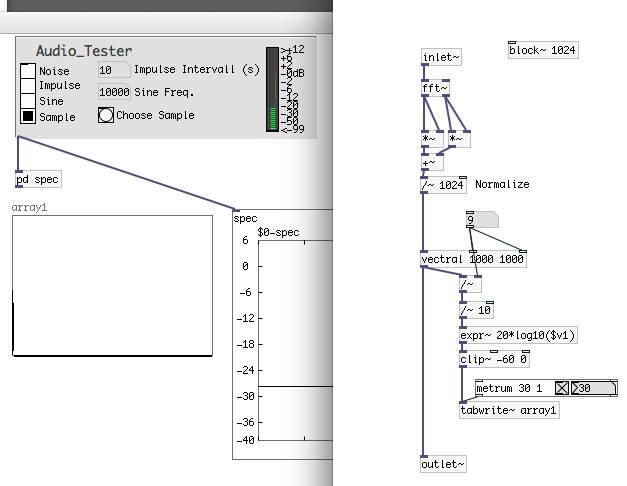
\includegraphics[width = 14cm]{img/showspectrum.png}
		\caption{showspectrum}
		\label{fig:showspectrum}
	\end{center}
\end{figure}
